%----------------------------------------------------------------------------------------
%	PACKAGES AND DOCUMENT CONFIGURATIONS
%----------------------------------------------------------------------------------------

\documentclass[
	a4paper, % Paper size, specify a4paper (A4) or letterpaper (US letter)
	10pt, % Default font size, specify 10pt, 11pt or 12pt
]{report}

\usepackage[utf8]{inputenc} % UTF-8 encoding
\usepackage[english]{babel} % Document language - required for customizing section titles
\usepackage{hyperref} % For hyperlinks
\hypersetup{
    colorlinks=false
}

\usepackage{geometry}
\geometry{top=3cm} % Adjust the top margin as needed
\geometry{bottom=2.8cm} % Adjust the bottom margin as needed

\usepackage{graphicx} % Required for the inclusion of images

\usepackage{caption} % Required for the inclusion of captions
\captionsetup{format=plain} % Removes any additional formatting after caption

\usepackage{float} % Allows putting an [H] in \begin{figure} to specify the exact location of the figure
\usepackage{booktabs} % Required for better horizontal rules in tables

\usepackage{amsmath, amssymb, amsthm} % Required for some math elements
\usepackage{siunitx} % Required for alignment of numbers with units

\usepackage{titlesec} % For custom section numbering format
\renewcommand{\thesection}{\arabic{section}} % Custom section numbering format (without prefix)

% \usepackage{biblatex} % Required for bibliography management
% \addbibresource{main.bib} % Bibliography file (located in the same folder as the main)


%----------------------------------------------------------------------------------------

\begin{document}

	%----------------------------------------------------------------------------------------
	%	REPORT INFORMATION
	%----------------------------------------------------------------------------------------

		\begin{titlepage}
		\centering
		\vspace{1.5cm} % Adjust vertical space

			
\includegraphics[width=1\textwidth]{figures/unimi.jpg} % University logo

		\vspace{1.5cm}
			
			\Huge Lab Report: \\ Differentiator and Integrator Circuits % Report title
			
		\vspace{1cm}
			
			\Large Lorenzo \textsc{Liuzzo} % Author name(s), add additional authors like: '\& James \textsc{Smith}'
			
		\vspace{2cm}
		
			\begin{tabular}{l r}
			
				Bachelor's Degree: & Physics \\ % Degree
				Course: & Electronics Laboratory \\ % Course
				Academic Year: & 2022/2023 \\ % Accademic year
				\\
				Instructor: & Professor Valentino \textsc{Liberali} \\ % Instructor/supervisor
				Partners: & Jiahao \textsc{Miao} \\ & Riccardo \textsc{Salto} \\ % Partner names
				\\
				Date Performed: & May 3, 2023 \\ % Date the experiment was performed
				
			\end{tabular}

		\vfill % Fill the rest of the page with whitespace
		\end{titlepage}


	%----------------------------------------------------------------------------------------
	%	ABSTRACT & TOC
	%----------------------------------------------------------------------------------------

		\abstract
In the realm of electronics and signal processing, a profound understanding of circuit behavior is paramount for designing high-efficiency systems. 
The primary objective of this experiment was to delve into the intricacies of differentiator and integrator circuits, shedding light on their frequency responses.
To achieve this, custom-tailored circuits were meticulously constructed to fulfill the distinct roles of measuring rate of change and cumulative input. 
Through comprehensive frequency sweeps that encompassed a spectrum from low to high frequencies, intricate data regarding gain and phase behaviors were collected and systematically scrutinized, 
revealing distinct patterns and behaviors across different frequency ranges. 

		{\let\clearpage\relax \tableofcontents}
		

	%----------------------------------------------------------------------------------------
	%	SECTIONS
	%----------------------------------------------------------------------------------------
		
		\clearpage % Forces the first chapter to start on an odd page so it's on the right

		\section{Introduction}
    %%% some intro stuff

    \subsection{Resistor-Transistor Logic}
        Resistor-Transistor Logic (RTL) is a fundamental digital logic family extensively used in electronic circuit design. 
        It leverages transistors for logic gates and integrates resistors for biasing and signal conditioning. 
        This straightforward and cost-effective approach to building digital circuits lays the groundwork for advanced logic families and integrated circuits. 

    \subsection{Bipolar Junction Transistor}
        The Bipolar Junction Transistor (BJT) is comprised of three layers: the emitter, the base, and the collector. 
        N-type and P-type materials, each doped with different impurities, compose these layers. 
        The emitter and collector are doped oppositely, either with excess electrons or holes, while the base remains lightly doped. 
        This setup creates two types of BJTs: NPN and PNP, defined by the arrangement of the layers.
        \begin{figure}[H]
            \centering
            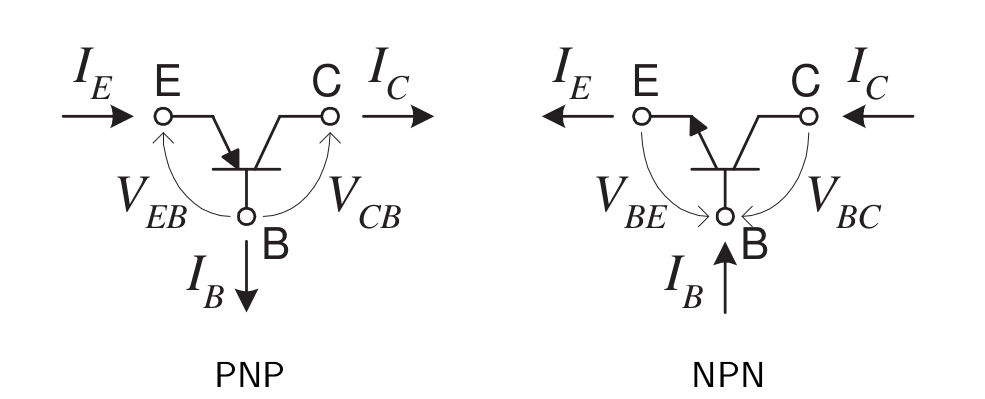
\includegraphics[width=0.7\textwidth]{figures/PNP_NPN.png}
            \caption{PNP and NPN Bipolar Junction Transistors}
            \label{fig:PNP_NPN}
        \end{figure}
        \noindent
        In its off state, the BJT functions as a switch, effectively isolating the collector from the emitter. 
        This behavior is consistent for both NPN and PNP BJTs. During this state, the collector-emitter junction acts as a barrier, preventing any significant current flow, much like a dam restraining water. 
        Additionally, the base-emitter junction remains non-conductive, blocking the flow of current from the emitter to the collector. \\
        Transitioning to the active state, the BJT takes on the role of a signal amplifier. A small current flows from the emitter to the base, giving rise to a more substantial current that courses from the collector to the emitter. 
        This relationship between the base and collector currents forms the cornerstone of the BJT's amplification capability. \\\\
        This amplification phenomenon hinges on the controlled movement of charge carriers across the emitter-base junction. 
        As electrons (or holes) traverse this junction, they engage with the majority carriers in the adjacent layer, resulting in the creation of localized charge regions. 
        These regions facilitate the flow of current from the collector to the emitter. \\
        In the NPN BJT, electrons cross from the emitter to the base. 
        The thinness of the base region and the attractive force exerted by the positively doped collector allow some electrons to overcome the barrier and reach the collector. 
        The modest base current exerts a substantial influence, enabling small variations in its magnitude to produce significant changes in the collector current. \\
        Similarly, the PNP BJT witnesses the flow of holes from the emitter to the base, and the base current governs the larger collector current. 
        In this configuration, the base-emitter junction, now comprised of N-type emitter material and P-type base material, emulates the behavior exhibited by the NPN counterpart. 
        Holes traverse the base region, ultimately converging at the collector, thus amplifying the overall current. \\\\
        As we increase the base current, a point is reached where the collector current can't increase further, regardless of the base current's rise. 
        This state is called saturation. It's as if the BJT switch is turned on fully, allowing maximal current flow through the collector-emitter path. \\
        On the opposite side, as the base current drops, the collector current also decreases until it nearly vanishes. 
        This state is known as cutoff, where the BJT operates as a near-perfect insulator, stopping any significant current from flowing through the collector-emitter junction.
        
    \subsection{Boolean Algebra}        
    

		\begin{samepage}
			\section{Equipment}
The experimental setup consists of the following components:

\begin{itemize}
    
    \item \emph{Bread-board}
	\item Probe and coaxial cables
	\item Resistor (\SI{9.94}{\kilo\ohm})
	\item Capacitor (\SI{2.27}{\nano\farad})
    \item Operational Amplifier (Op-Amp uA741): used to amplify the voltage difference between its input terminals.    
    \item Power supplies: provide the necessary voltage levels for the Op-Amp.
    \item Signal generator Agilent 33220A: provides the input voltage signal.
    \item Oscilloscope Tektronix TDS2012C: used to measure and visualize the input and output waveforms and their time shift.

\end{itemize}

			\section{Procedure}
The following steps were undertaken to conduct the experiment:

\begin{enumerate}

    \item \textbf{Frequency Setup}: 
    Begin by setting the desired frequency of the input signal using the function generator. It is advised to follow a logarithmic scale
    
    \item \textbf{Input Signal Configuration}: 
    Configure the input signal to align with the chosen frequency and amplitude specifications. Opt for a sinusoidal waveform as input signal. 
    Using the BNC T-splitter establish the connection between the configured signal and the circuit's input and oscilloscope.
    
    \item \textbf{Output Signal Measurement}: 
    Employ an oscilloscope to measure the output signal of the circuit. Connect the oscilloscope to the circuit's output to visualize its response to the input signal.
    
    \item \textbf{Voltage Measurement Across Resistor (Differentiator Circuit)}: 
    For the differentiator circuit, measure the voltage across the resistor using the oscilloscope. 
    
    \item \textbf{Voltage Measurement Across Capacitor (Integrator Circuit)}: 
    For the integrator circuit, introduce an additional resistor in parallel with the capacitor to incorporate an offset voltage and measure the voltage across the capacitor using the oscilloscope. 
    
    \item \textbf{Time Difference Measurement}: 
    Further analyze the phase shift between the input and output signals by measuring the time difference between corresponding points on the two signals using the oscilloscope's cursors.
    
    \item \textbf{Gain Calculation}: 
    Calculate the gain of the circuit in decibels (dB) using the formula: $$ \text{Gain}_{\text{dB}} = 20 \log_{10} \left( \frac{V_{\text{out}}}{V_{\text{in}}} \right) $$
    where $V_{\text{out}}$ represents the measured output voltage and $V_{\text{in}}$ is the input voltage.
    
    \item \textbf{Phase Shift Calculation}: 
    From the time difference measured, determine the phase shift between the input and output signals in radians through the formula:
    $$ \text{Phase shift (radians)} = 2\pi \cdot \text{Time difference} \cdot \text{Frequency}$$

\end{enumerate}

		\end{samepage}

		\section{Discussion}
The experimental investigation of the differentiator and integrator circuits' frequency response characteristics is presented in this section.
	
	\subsection{Experimental results}
		Bode plots, which graphically depict the gain and phase shift of a circuit over a range of frequencies, were employed to visualize these characteristics. \\\\
		Figures \ref{fig:differentiator_bode} and \ref{fig:integrator_bode} showcase the Bode plots of the differentiator and integrator circuits, respectively.
		To generate these plots, data was extracted from a text file containing recorded frequency values along with their corresponding circuit gain (expressed in decibels) and phase shift (in radians). 
		The dataset used for each Bode plot is also included in the Appendix (Tables \ref{tab:differentiator_data} and \ref{tab:integrator_data}). \\\\
		A logarithmic scale is employed on the x-axis to cover the range of frequencies effectively. 
		The incorporation of dual y-axes facilitates the visual comprehension of the frequency response traits exhibited by the circuits: 
		the left y-axis is dedicated to displaying gain, while the right y-axis portrays phase shift.
		To enhance clarity, data is displayed with different color markers: blue for the gain and yellow for the phase shift.

		\begin{figure}[H]
		    \centering
		    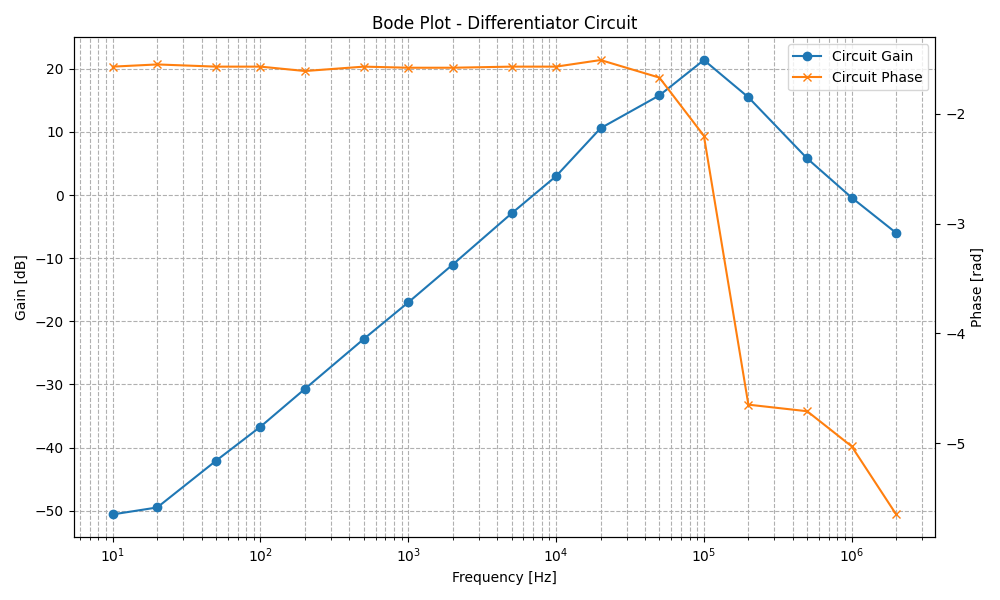
\includegraphics[width=1\textwidth]{figures/differentiator/bode_plot.png}
		    \caption{Bode plot for the differentiator circuit.}
		    \label{fig:differentiator_bode} 
		\end{figure}


		\begin{figure}[H]
		    \centering
		    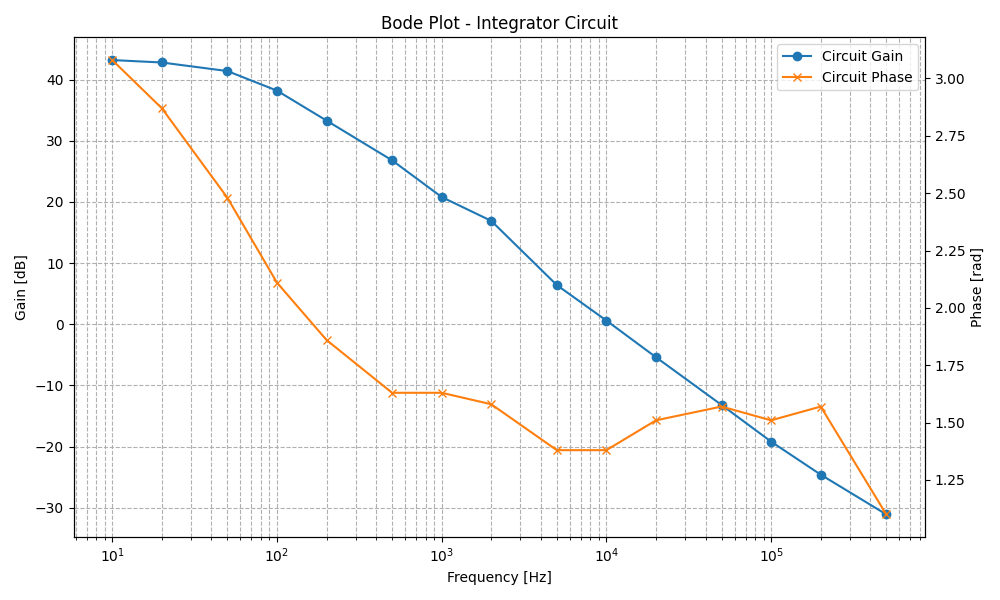
\includegraphics[width=1\textwidth]{figures/integrator/bode_plot.png}
		    \caption{Bode plot for the integrator circuit.}
		    \label{fig:integrator_bode}
		\end{figure}
	
	% comment of the Figures


	\subsection{Simulated results}
	   
		To delve deeper into the analysis of our experimental findings, the differentiator and integrator circuits were simulated using ngspice, a renowned simulation tool based on the Berkeley SPICE software. 
		This simulation process aimed to replicate the behavior of the electronic circuits under investigation. 
		The net-lists employed for simulating these circuits can be found in the Appendix for reference. \\\\
		Figures \ref{fig:differentiator_gain} and \ref{fig:differentiator_phase} provide a platform for comparing the experimental data with the corresponding simulated results for the differentiator circuit.
		Similarly, figures \ref{fig:integrator_gain} and \ref{fig:integrator_phase} present a comparative analysis between experimental and simulated data for the integrator circuit. \\
		
		\begin{figure}[H]
		    \centering
		    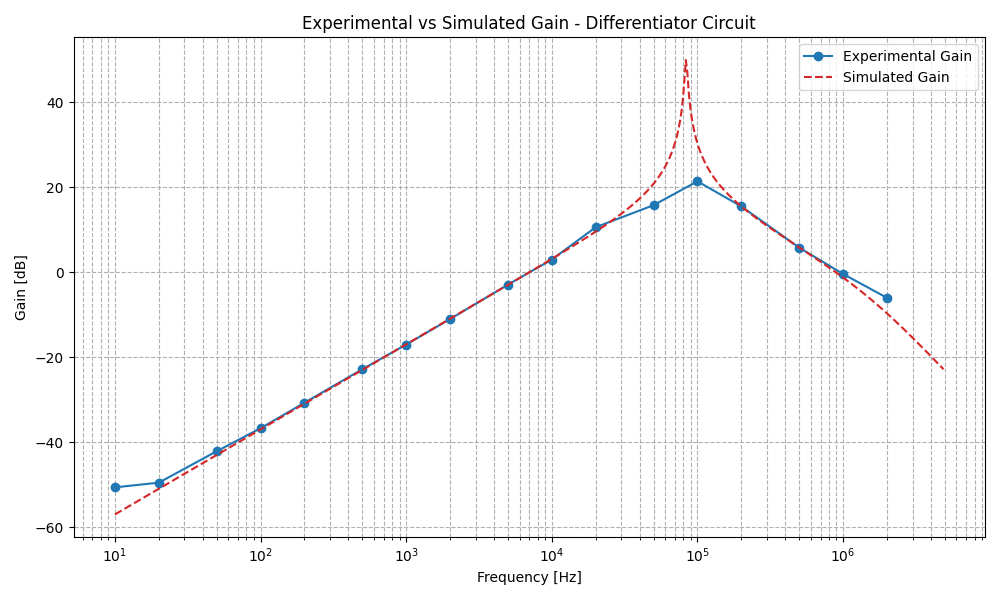
\includegraphics[width=1\textwidth]{figures/differentiator/gain_plot.png}
		    \caption{Gain comparison between experimental and simulated data for the differentiator circuit.}
		    \label{fig:differentiator_gain}
		\end{figure}

		\begin{figure}[H]
		    \centering
		    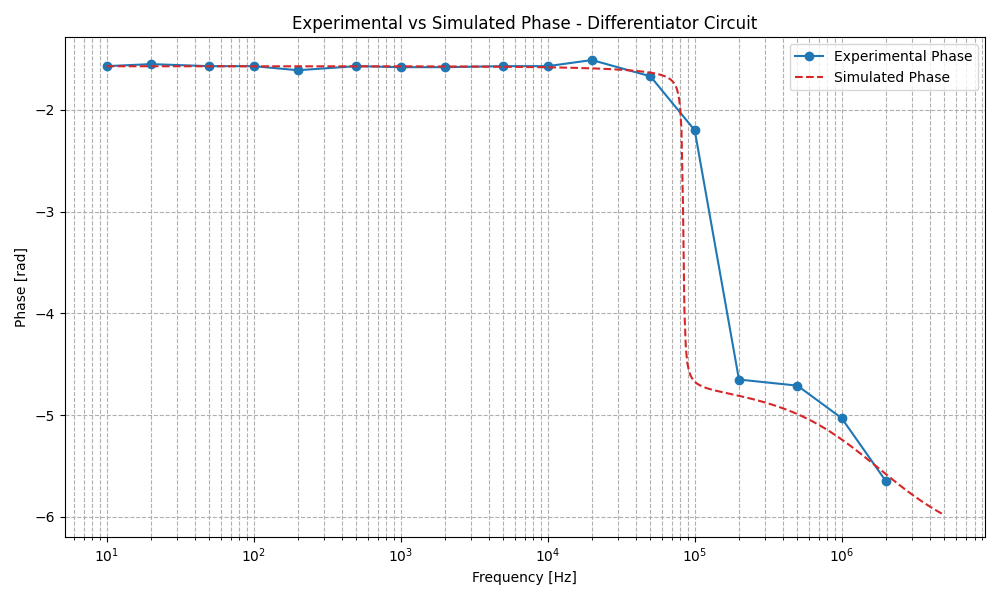
\includegraphics[width=1\textwidth]{figures/differentiator/phase_plot.png}
		    \caption{Phase comparison between experimental and simulated data for the differentiator circuit.}
		    \label{fig:differentiator_phase}
		\end{figure}

		\begin{figure}[H]
		    \centering
		    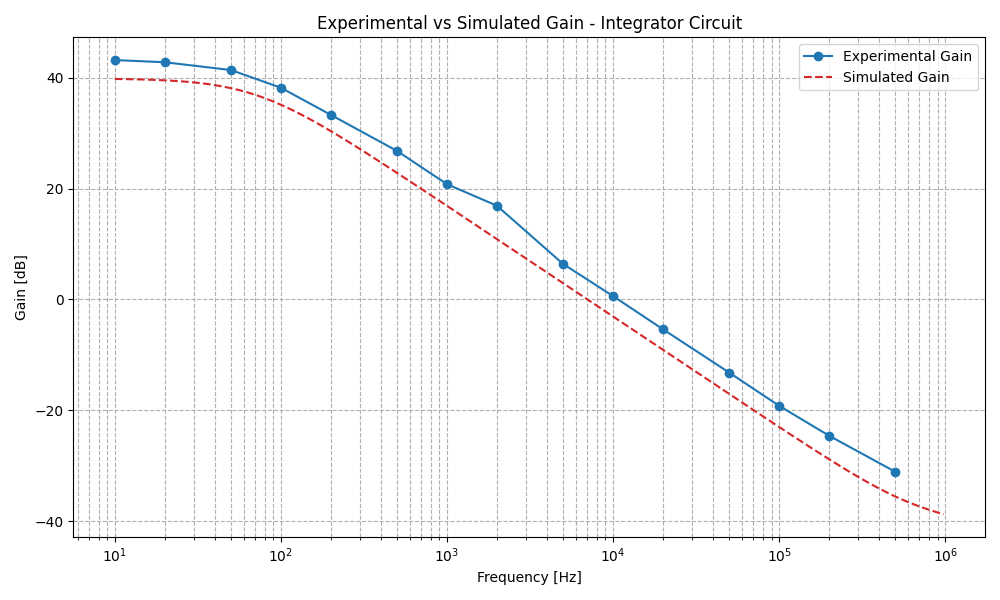
\includegraphics[width=1\textwidth]{figures/integrator/gain_plot.png}
		    \caption{Gain comparison between experimental and simulated data for the integrator circuit.}
		    \label{fig:integrator_gain}
		\end{figure}

		\begin{figure}[H]
		    \centering
		    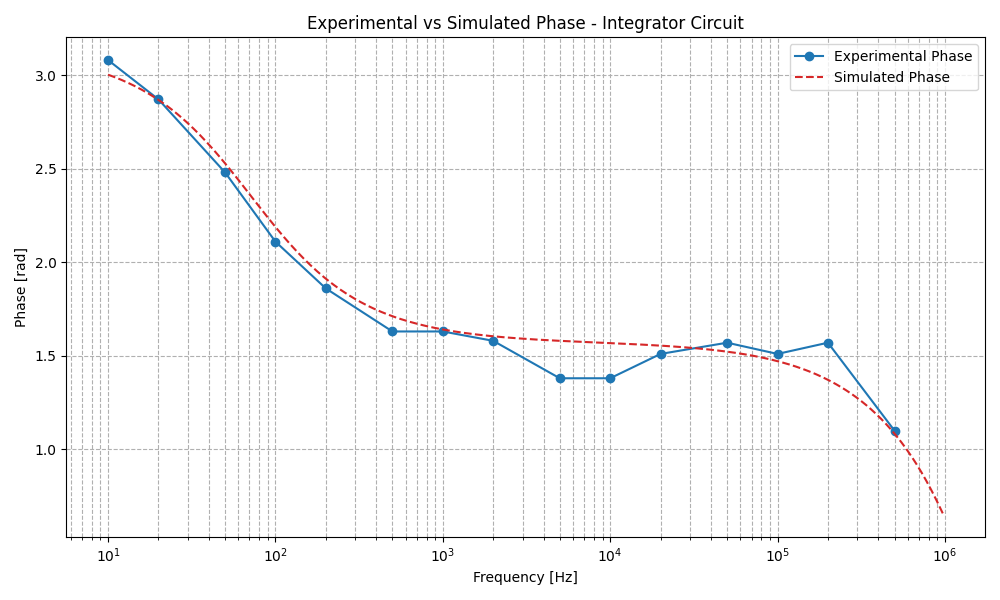
\includegraphics[width=1\textwidth]{figures/integrator/phase_plot.png}
		    \caption{Phase comparison between experimental and simulated data for the integrator circuit.}
		    \label{fig:integrator_phase}
		\end{figure} 

		The alignment between our real-world tests and simulated results demonstrates the harmony between our theoretical predictions and observed outcomes, underscoring the accuracy of our hands-on methods.

		%\section{Conclusions}

		\appendix

\section*{Appendix}

\addcontentsline{toc}{section}{Appendix} % Add "Appendix" to the table of contents
		
		
	%----------------------------------------------------------------------------------------
	%	BIBLIOGRAPHY
	%----------------------------------------------------------------------------------------

		% \printbibliography % Output the bibliography


\end{document}

%----------------------------------------------------------------------------------------
